\documentclass[twoside, single, authoryear, semicolon]{lion-msc}
\usepackage{lipsum}
\usepackage{booktabs}
\usepackage[version=4]{mhchem}

\title{Identifying Nitrogen Carriers in Planet-Forming Regions of Protoplanetary Disks}
\author{Niels de Klerk}

\major{Astronomy and Physics}
\affiliation{Leiden Observatory, Universiteit Leiden}

\newdate{date}{\day}{\month}{\year}           % definition of time and date using datetime package
% \newdate{date}{27}{08}{2010}
\date{\displaydate{date}}

\studentid{s3640477}                           % check you student ID, LaTeX does not do this
\abstract{Here goes a wonderful abstract.}   % limit your self to 1/2 page or 500 words
\dailysupervisor{Msc. Marissa Vlasblom \\ \hspace*{\fill}Msc. Aditya Arabhavi}
\supervisor{Prof. Dr. Ewine van Dishoeck \\ \hspace*{\fill}Prof. Dr. Inga Kamp} % Note that this should be a LION staff member!
\corrector{Dr. Matthieu Schaller}                      % This could be a LION staff member or your external supervisor

\degree{Bachelor of Science}                     % The default option is "Bachelor of Science", change if needed

\major{Astronomy and Physics}                  % The default option is "Physics", change if needed
%\major{Physics and Mathematics}

% optional cover picture - should be jpg or pdf
% \coverpicture{
\includegraphics[width=10cm]{Latex/lion-msc-logo.pdf}}

% Use this to make hyperlinks visible in the document.
% \hypersetup{colorlinks=true}

% ---------------------------------------------------------------- My defintions!
% \renewcommand{\vec}[1] {\ensuremath{ \overrightarrow{ #1 } }}
\renewcommand{\vec}[1] {\ensuremath{ \mathbf{ #1 } }}
% \bra \ket \braket and \proj
\newcommand{\bra}[1]{\ensuremath{\langle #1 \vert}}
\newcommand{\ket}[1]{\ensuremath{\vert #1 \rangle}}
\newcommand{\braket}[2]{\ensuremath{\langle #1 \vert #2 \rangle}}
\newcommand{\proj}[1]{\ensuremath{\vert #1 \rangle \langle #1 \vert}}

\newcommand{\kpar}{\ensuremath{k_\parallel}}

\newcommand{\3}{$_3$}
\newcommand{\2}{$_2$}
% ----------------------------------------------------------------

% \usepackage{tocloft}
% \renewcommand{\cftchapdotsep}{\cftdotsep}
\begin{document}

% roman numbering in the table of contents section
\pagenumbering{roman}

\maketitle

% Table of contents:  it is a good idea to include this into your thesis
\tableofcontents
\cleardoublepage
\pagenumbering{arabic}
\chapter{Introduction}
The nebular hypothesis was first proposed in \textit{The Principia} by Emanuel Swedenborg in 1745. Immanuel Kant developed the theory further in 1752 and it was modified by Pierre-Simon Laplace in 1796. The theory states that a planetary system is formed from a slowly rotating gas cloud, which collapses down into a disk. Centuries later, the first protoplanetary disk was observed by O'Dell using the Hubble Space Telescope \citep{ODell1993}. In recent years, the Atacama Large Millimeter/submillimeter Array (ALMA) has imaged a large collection of these protoplanetary disks, showing a wide variety of structures and compositions. The JWST MIRI mid-INfrared Disk Survey (MINDS) team uses the JWST to investigate the inner parts of protoplanetary disks. The study of protoplanetary disks is important to find answers to the fundamental questions, 'How did life arise?' and 'Are we alone in the universe?'.

The spectrum of protoplanetary disks can tell us a lot about the properties of the disk and the host star. An important example is an observation of the disk around a T Tauri star 89sz \citep{Gasman_2023}. Using MIRI on the JWST, they probed the inner regions of the disk. They detected CO$_2$, H$_2$O, OH, CO, and HCN. Furthermore, no other organics were detected, suggesting a low C/O ($<$0.5) ratio. This result differed from the ratio found using ALMA ($>$1), which probed the outer regions. This highlights the complexity of disks and their chemistry.

However, this observation is not necessarily representative of disks. \cite{colmenares2024jwstmiridetectioncarbonrichchemistry} observed a disk around the T Tauri star DoAr 33 with an exceptionally high C/O ratio of 2-4. In addition to CO, H$_2$O, and CO$_2$ like in the 89 sz disk, the more complex carbohydrates C$_2$H$_2$ and C$_4$H$_2$ were found. The presence of these molecules is indicative of this high ratio. A possible explanation for this carbon-rich environment is the slow accretion rate of the star, which results in slowing the radial mixing and the persistence of the carbon-grain destruction.

Observations of the protoplanetary disk around the T Tauri star GW lup have given the first detection of $^{13}$CO$_2$ in a protoplanetary disk. \cite{Grant_2023} The combination with the spectral resolution of the JWST-MIRI and the high SNR allows for the detection of weaker spectral features. Notably, the deduced N$_{CO_2}$/N$_{H_2O}$ was significantly higher than previously thought. This could indicate a cavity between the H$_2$O and CO$_2$ snowlines. These findings show the new possibilities JWST provides for studying disk structures. 

The effects of a cavity on the spectrum were studied by \cite{vlasblom2023midinfraredspectrattauri}. It was speculated that 'CO$_2$-only sources' have inner cavities which extend beyond the H$_2$O snowline, but stay within the CO$_2$ snowline. By running thermo-chemical models with different inner cavity sizes it was shown that N$_{CO_2}$/N$_{H_2O}$ grows as the size of the cavity grows and then sharply drops. The conclusions drawn from this can help to interpret the spectra of disks.

In chapter \ref{Ch: Theoretical Background} we give background information about processes in the protoplanetary disks and simulations. We present the data and the methodology in chapter \ref{Ch: Methods}.



\section{Formation and evolution of Disks}
Molecular clouds are large collections of gas and dust. When these clouds are perturbed, parts of the cloud can become dense enough, making them collapse under their gravity. This will result in the creation of a star surrounded by gas and dust. The angular momentum of each of the particles is randomly oriented, but on average the angular momentum vector is pointed in a certain direction. Two particles colliding will cause them to exchange angular momentum. If many collisions happen, all the angular momenta of the other than the average angular momentum vector get canceled out. This results in the formation of a disk around the pre-main-sequence star.
The evolution of the disk can be categorized into 4 classes \citep{1987ApJ...312..788A}. Class 0 are objects where an optically thick envelope surrounds the protostar. Class I objects have a star and disk but are still embedded in an optically thick envelope. The star and disk become visible in class II objects as the star has become bright enough to blow away the envelope. In class III objects, the disk has largely been depleted of gas and dust, leaving behind planets and planetesimals. 
% Factors that influence the evolution



The protoplanetary disk has structure, namely the radial structure and the vertical structure. The innermost regions ($<$10 AU) of the disk are the hottest and receive the most radiation. Most of the molecules are in gaseous form in this region, except for some silicates and metals. The star heavily influences the chemistry. The intermediate regions (10-100 AU) have lower temperatures, allowing molecules like water to condense. The outer regions ($>$100 AU) are the coldest in the disk. Molecules have formed ice here making them inert. \\
The height of the disk is also an important factor in its structure. The midplane is the horizontal plane through the center of the disk. Most dust particles settle around the midplane whereas the gas particles are further out. The midplane is also colder than the outside of the disk as it receives less light from the star. The protoplanetary disk tends to flare outwards. Close to the star the disk is fairly compact, but when you go outwards from the star, the disk gets more and more extended from the midplane. 

\begin{figure}[!ht]
    \centering
    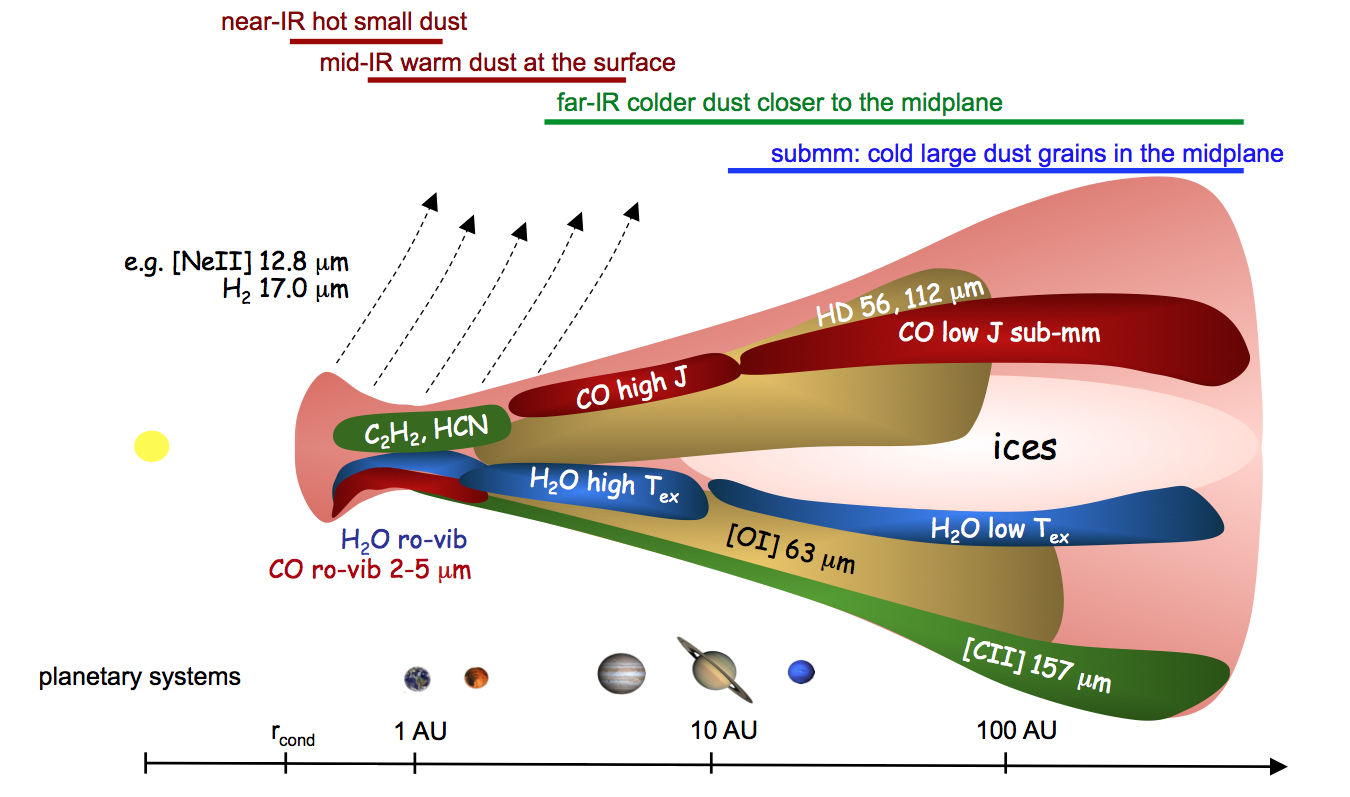
\includegraphics[width=\linewidth]{Figures/disk-sketch.png}
    \caption{A schematic representation of a protoplanetary disk. The planets in the solar system are shown as a point of reference. \cite{inproceedings}}
    \label{fig:enter-label}
\end{figure}

\section{Disk Chemistry}

\section{Emission Mechanisms}

\section{JWST MIRI MRS}

% \section{Radiative Transfer}
\section{Modeling}
Some of the properties of the protoplanetary disks can be directly inferred from disk measurements. For instances where this is not the case, we would still like to learn more from our data via a different method. We can use models to simulate the protoplanetary disk and generate synthetic data to compare to actual observations. There are various types of models. Ranging from 1D slab models to thermo-chemical disk models. For our research, we run simulations using PROtoplanetary DIsk MOdel (ProDiMo), a thermo-chemical disk model. The output of those simulations is then put through Fast Line Tracing system (FLiTs) to get an accurate spectrum of the disk. 
\section{Goal}

\chapter{Methods}\label{Ch: Methods}
\section{ProDiMo Simulations}

\begin{table}[!h]
\centering
\begin{tabular}{@{}lll@{}}
                                  &                             &                            \\ \hline\midrule
\textbf{Property}                 & \textbf{Symbol}             & \textbf{Value}             \\ \midrule
Stellar mass                      & M$_\ast$                    & 0.7M$_\odot$               \\
Effective Temperature             & T$_\ast$                    & 4000 K                     \\
Stellar Luminosity                & L$_\ast$                    & 1 L$_\odot$                \\
UV excess                         & f$_{UV}$                    & 0.01                       \\
UV powerlaw index                 & p$_{UV}$                    & 1.3                        \\
X-ray luminosity                  & L$_x$                       & 10$^30$ erg/s              \\
X-ray emission temperature        & T$_x$                       & 2$\times10^7$ K            \\ \midrule
Strength of interstellar UV       & $\chi^{ISM}$                & 1                          \\
Strength of interstellar IR       & $\chi^{ISM}_{IR}$           & 0                          \\
Cosmic ray H$_2$ ionization rate & $\zeta_{CR}$                & $1.7\times10^{-17} s^{-1}$ \\ \midrule
Inner disk radius                 & R$_{in}$                    & 0.05 au                    \\
Outer disk radius                 & R$_{tap}$                   & 30 au                      \\
Column density power index        & $\epsilon$                  & 1                          \\
Reference scale height            & H$_g$ (100 au)              & 10 au                      \\
Flaring power index               & $\beta$                     & 1.15                       \\ \midrule
Minimum dust particle radius      & a$_{min}$                   & 0.05 $\mu$m                \\
Maximum dust particle radius      & a$_{max}$                   & 3000 $\mu$m                \\
Dust size dist. power index       & a$_{pow}$                   & 3.5                        \\
Turbulent mixing parameter        & $\alpha_{settle}$           & 0.001                      \\
Refractory dust composition       & Mg$_{0.7}$Fe$_{0.3}$SiO\3 & 60 \%                      \\
                                  & amorph. C                   & 15 \%                      \\
                                  & porosity                    & 25 \%                      \\
PAH abundance rel. to ISM         & f$_{PAH}$                   & 0.01                       \\
Chemical heating efficiency       & $\gamma^{chem}$             & 0.2                        \\ \midrule
Distance to the observer          & d                           & 140 pc                     \\ \bottomrule
\end{tabular}
\caption{}
\label{tab:parameters}
\end{table}

We ran a model grid with varying abundances of C and O using ProDiMo. The parameters with which the models were run are in table \ref{tab:parameters}. The abundances of C and O were varied between -0.5 and 0.5 in steps of 0.25, where 0 corresponds to the solar abundance. The grid contains 25 models, with the fiducial model in the middle, which is based on the solar abundances of C and O.

\begin{table}[!h]
\centering
\begin{tabular}{@{}lll@{}}
                                  &                             &                            \\ \hline\midrule
\textbf{Element} & \textbf{+12 Abundance} & \textbf{Variation}            \\ \midrule
H                & 12                     & Fixed                         \\
He               & 10.984                 & Fixed                         \\
C                & 8.140                  & {[}-0.5, -0.25, 0, +0.25, +0.5{]} \\
N                & 8.900                  & Fixed                         \\
O                & 8.480                  & {[}-0.5, -0.25, 0, +0.25, +0.5{]} \\
Ne               & 7.950                  & Fixed                         \\
Na               & 3.360                  & Fixed                         \\
Mg               & 4.030                  & Fixed                         \\
Si               & 4.240                  & Fixed                         \\
S                & 5.270                  & Fixed                         \\
Ar               & 6.080                  & Fixed                         \\
Fe               & 3.240                  & Fixed                         \\
PAH              & 3.444                  & Fixed                         \\ \bottomrule
\end{tabular}
\caption{}
\label{tab:abundances}
\end{table}



After running the model grid, we used FLiTs to generate the spectra for all the models. We calculated the entire spectrum containing  \textbf{INSERT EXACT MOLECULES IN THE TOTAL SPECTRUM} and the spectra of individual molecules as well. The spectra we retrieved with FLiTs have an unrealistically high resolution. To make the spectrum more realistic, we convolved the spectrum to a resolving power of 3000 using the \textit{prodimopy.read.DataFLiTsSpec.convolve}\citep{SOURCE}, which convolves the spectrum with a Gaussian kernel to create a spectrum of the correct resolving power. The value of 3000 was chosen as it is approximately the average resolving power of the MIRI MRS \citep{SOURCE}. 

We wanted to add noise to the data to make the simulated spectra as realistic as possible. The MINDS team has observations which have $SNR = 300$ \citep{SOURCE}. We want to make our simulated data follow the same vein. Using the spectrum minimum, we estimate the noise level needed to create an $SNR = 300$. We assume that the noise is normally distributed. After applying this noise, we subtract the continuum to get the actual spectrum we can use to analyse the different molecules that compose it.


The flux density we have from FLiTs is in units of Jansky, but we would like to integrate the flux density to get the flux. For this, we need to convert the flux per unit frequency to flux per unit wavelength. We use the equation

\begin{equation}
    F_\lambda=\frac{c}{\lambda^2}F_\nu
\end{equation}

\textbf{SPECTRUM CLASSIFICATION}

\section{Cross-Correlation}
For our analysis, we used cross-correlation. This is a signal detection technique for detecting weak signals. It is defined as follows. 
\begin{equation}
    R_{fg}(\tau)=\int^\infty_{-\infty}\overline{f(t)}g(t+\tau)dt
\end{equation}
The autocorrelation is the cross-correlation of a function with itself
\begin{equation}
    R_{ff}(\tau)=\int^\infty_{-\infty}\overline{f(t)}f(t+\tau)dt
\end{equation}
As all our functions are real valued, we can omit the complex conjugation in the integrand.

We calculated the average spectrum for each species and divide that by the maximum of the spectrum to normalize it. We used this template spectrum to cross-correlate with the spectrum containing all the species. The cross-correlation should peak when the template spectrum matches with the spectrum containing all the species. To quantify the height of the peak, we calculated the difference between the height of the peak and the median value of the cross-correlation in a small region around the peak. We took the median as this is less susceptible to outliers to capture the general trend around the peak more optimally. We used hypothesis testing to test whether or not there is statistical evidence to say the molecule is present. We had the following null hypothesis and alternative hypothesis

\begin{equation}
    H_0: \text{The height of the peak in the cross-correlation is caused by noise}
\end{equation}
\begin{equation}
    H_1: \text{The height of the peak in the cross-correlation is caused by the molecule}
\end{equation}

To assess the significance of the peak in cross-correlation, we used a Monte Carlo simulation to simulate 10000 synthetic spectra under the null hypothesis. First, we take all the flux values we have for different wavelength values. Second, we sample with replacement from the flux values until we have a collection of values that is the same size as the original set. Third, we take the cross-correlation and calculate the difference between the height of the peak and the median value of the cross-correlation in a small region around the peak. The value of the original data is deemed significant when it exceeds 95\% of the values from the simulated data ($\alpha=0.05$).

\textbf{SOMETHING ABOUT REGIONS SELECTION}


\section{Observations}
After looking at the simulated spectra, we wanted to apply our techniques to observations made with JWST MIRI MRS. We have access to 3 sources. 
1D LTE models to fit the model and try to enhance the hidden molecules
\begin{figure}[!ht]
    \centering
    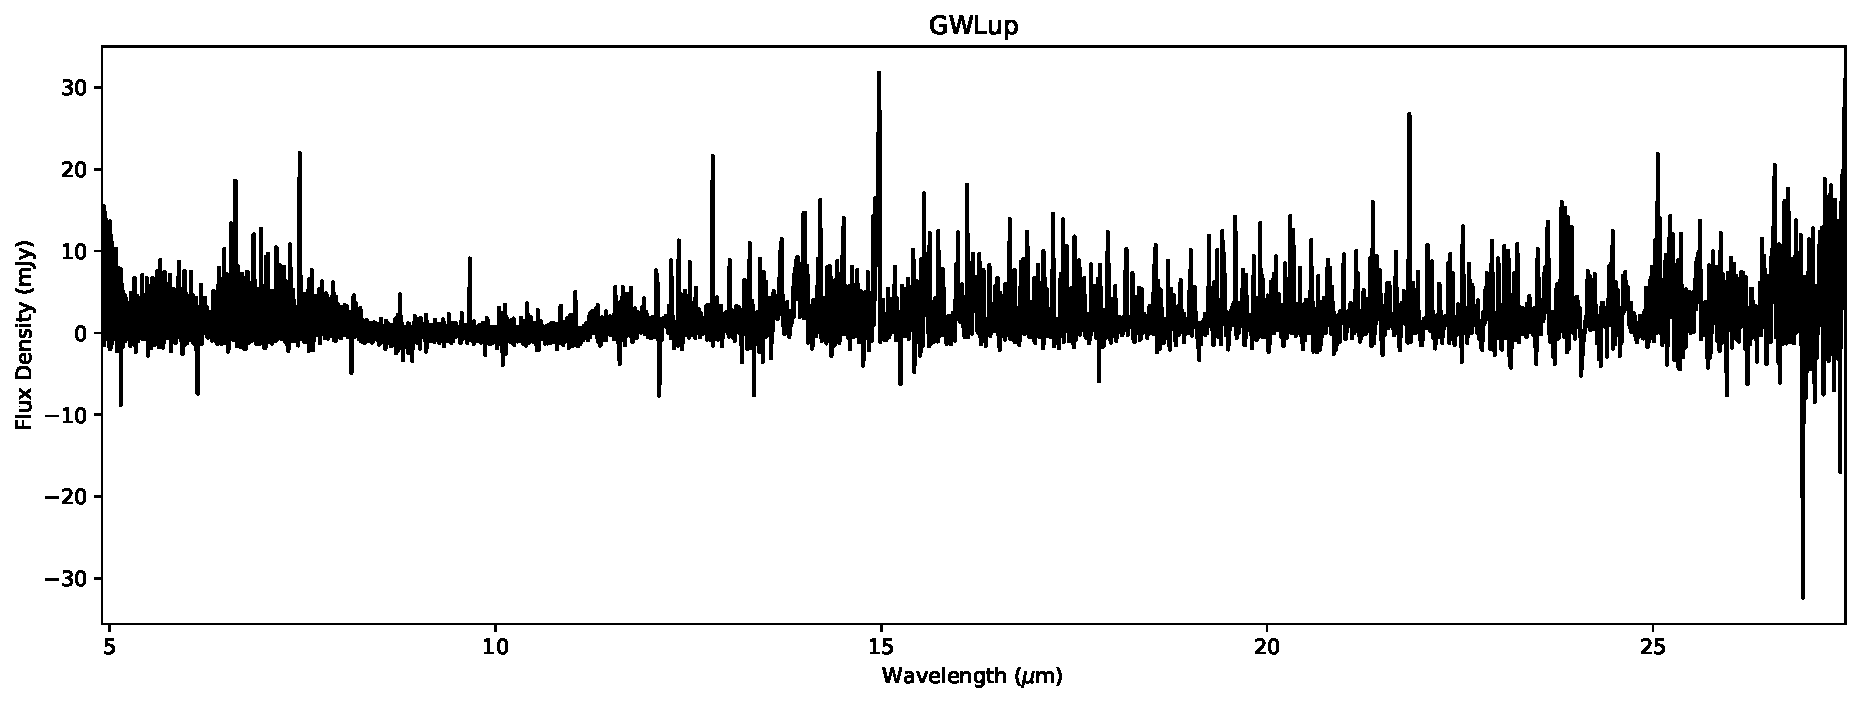
\includegraphics[width=\linewidth]{Figures/FullSpectrum_GWLup.pdf}
    \caption{The continuum subtracted spectrum of GWLup}
    \label{fig:GWLup}
\end{figure}
\begin{figure}[!ht]
    \centering
    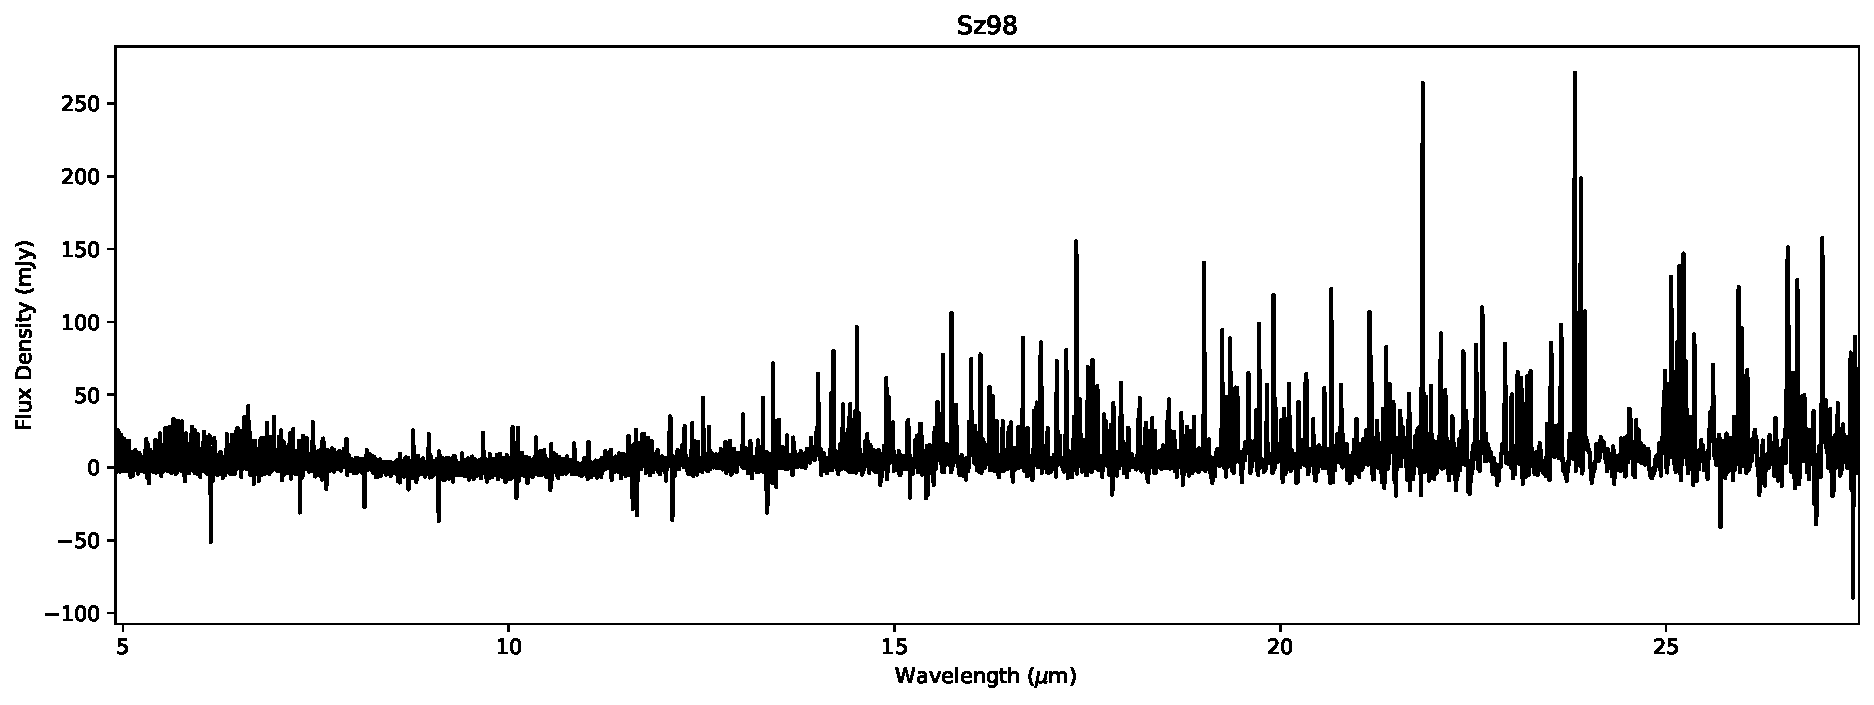
\includegraphics[width=\linewidth]{Figures/FullSpectrum_Sz98.pdf}
    \caption{The continuum subtracted spectrum of Sz98}
    \label{fig:Sz98}
\end{figure}
\begin{figure}[!ht]
    \centering
    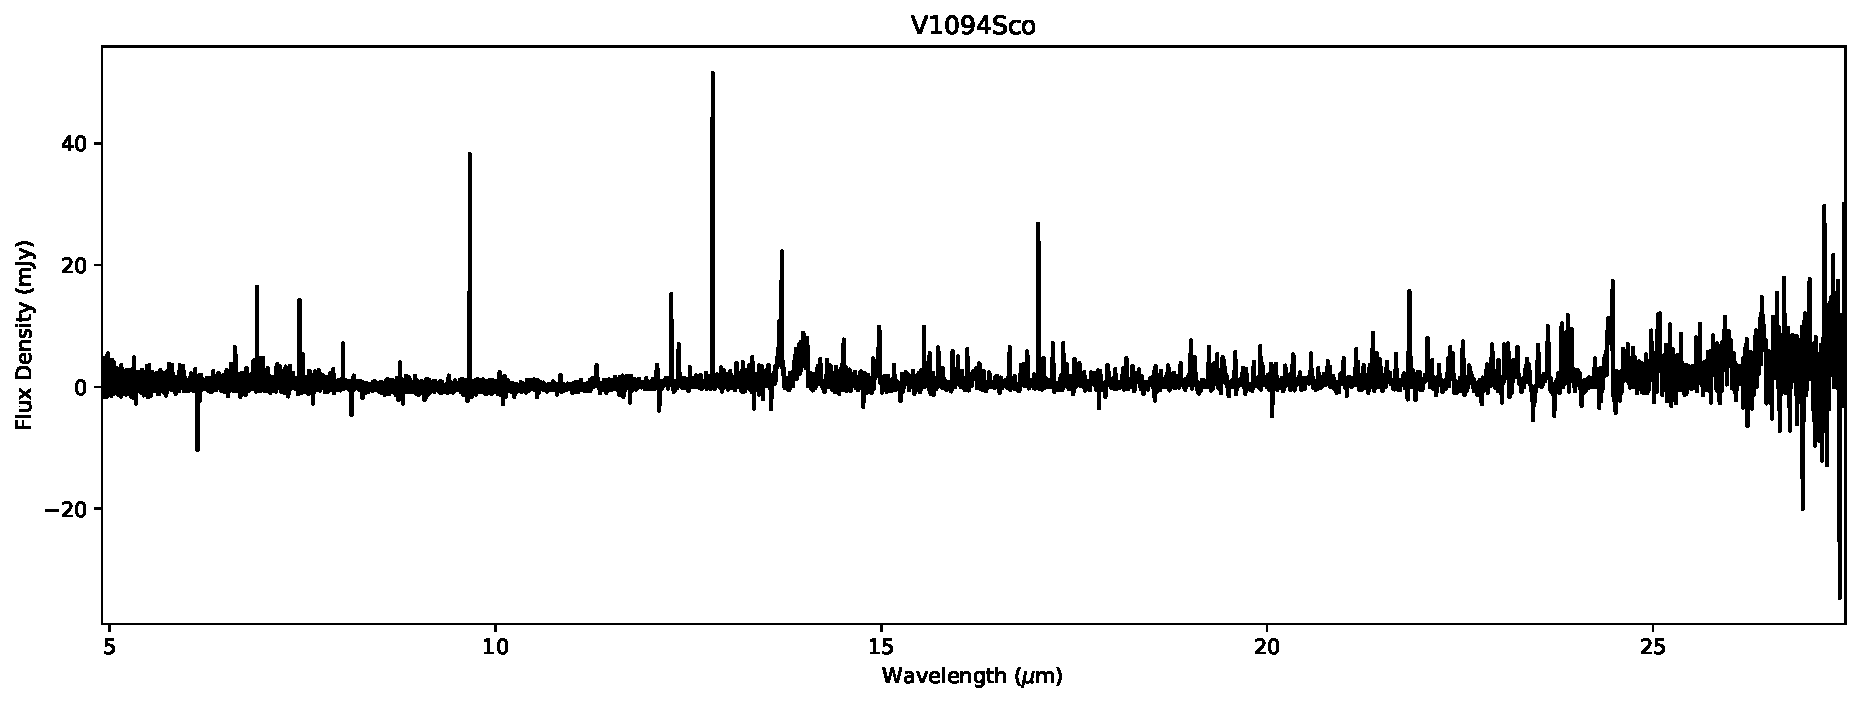
\includegraphics[width=\linewidth]{Figures/FullSpectrum_V1094Sco.pdf}
    \caption{The continuum subtracted spectrum of V1094Sco}
    \label{fig:V1094Sco}
\end{figure}



\chapter{Results}
\section{ProDiMo Output}
After running the models, we inspect their output. First, we look at the densities of the gas and dust in the disk. We see that the density of the gas stretches higher than the density of the dust. This is expected, as we know that the dust settles around the midplane. 

\begin{figure}[!ht]
    \centering
    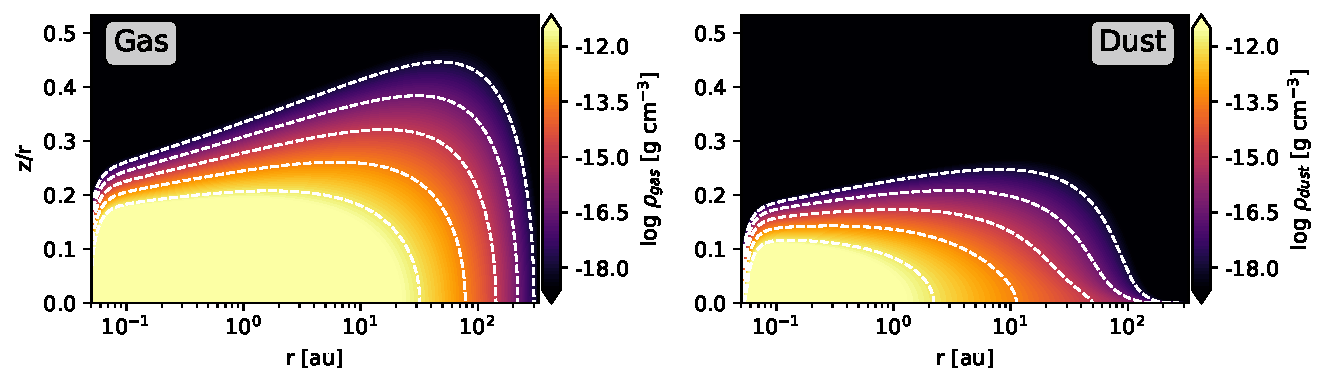
\includegraphics[width=\linewidth]{Figures/Density.pdf}
    \caption{The distribution of the gas and dust in the disk of the fiducial model.}
    \label{fig:density}
\end{figure}

Next, we inspect the temperature of the gas and dust across the disk. We can see is that the gas temperature is more structured around the midplane. The dust temperature gradient has straight sections above the main body of the disk. This result is also expected as the density of the dust is orders of magnitude lower in the regions above the disk. This results in the starlight getting barely blocked, so the temperature doesn't change across different heights.

\begin{figure}[!ht]
    \centering
    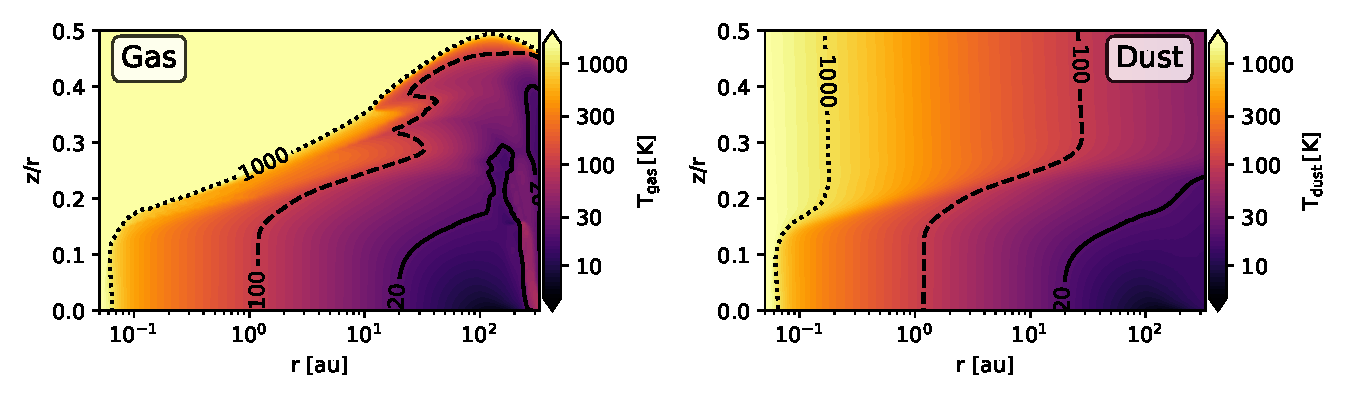
\includegraphics[width=\linewidth]{Figures/Temperature.pdf}
    \caption{The temperature of the gas and dust in the disk of the fiducial model.}
    \label{fig:temperature}
\end{figure}

Lastly, we inspect the distribution of HCN, HNC, NH\3, and NO -common nitrogen carriers. We see in figure \ref{fig:nitrogen distribution} that the density of the molecules changes a lot for different radii and heights. For example, in the region between 1, 2 we see that HCN decreases compared to the surrounding regions, but HNC increases in the same region. 

\begin{figure}[!ht]
    \centering
    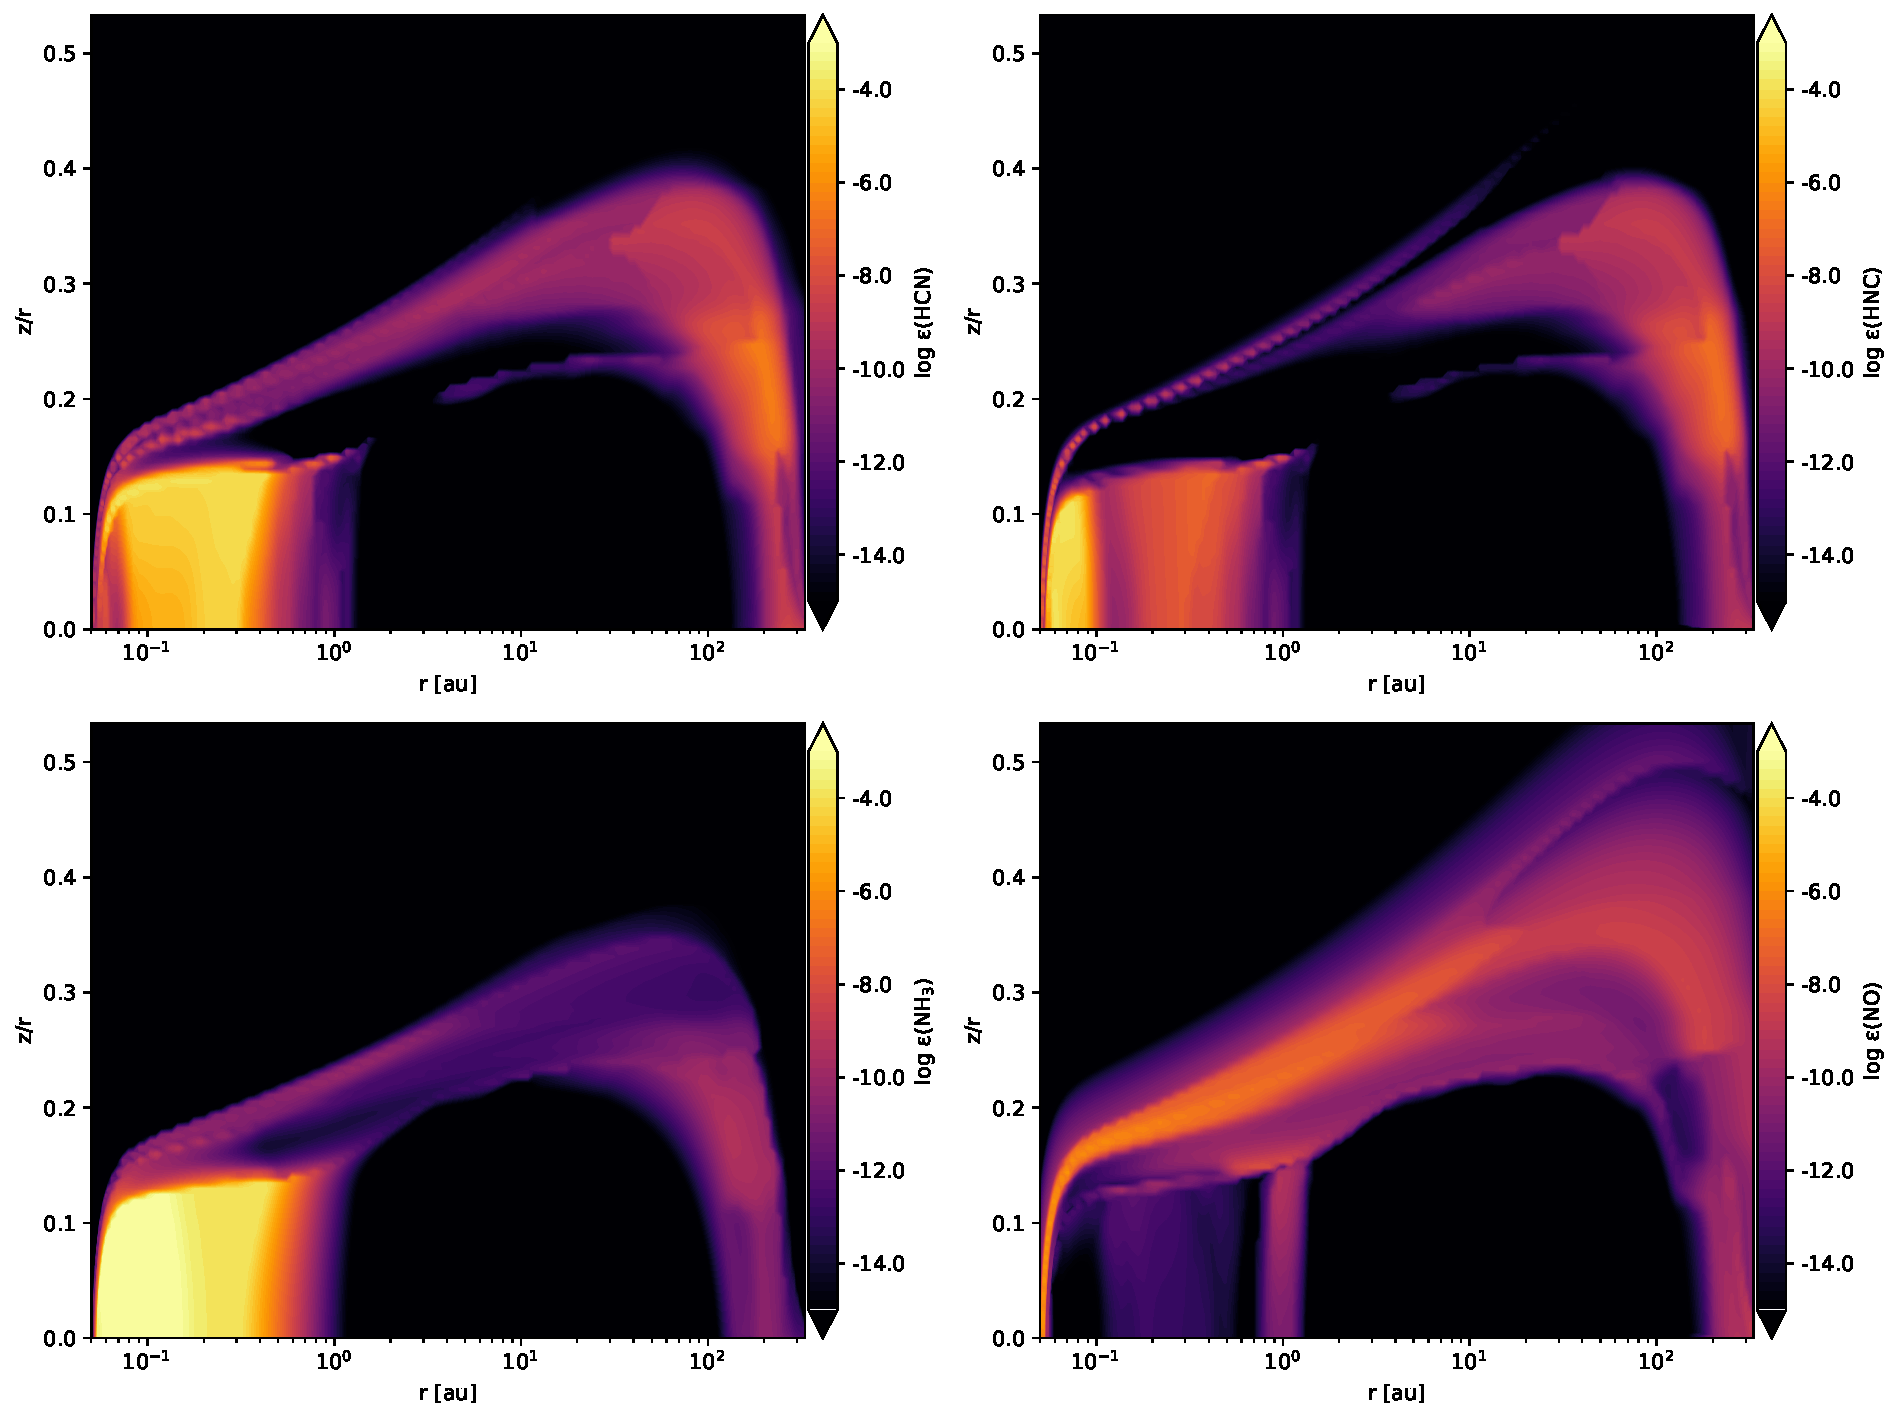
\includegraphics[width=\linewidth]{Figures/Abundance.pdf}
    \caption{The distribution of HCN, HNC, NH\3, and NO across the disk of the fiducial model.}
    \label{fig:nitrogen distribution}
\end{figure}
\section{FLiTs Spectra}
The models in the model grid we have created were used with FLiTs to create accurate spectra. The resulting spectra containing 
\begin{figure}[!h]
    \centering
    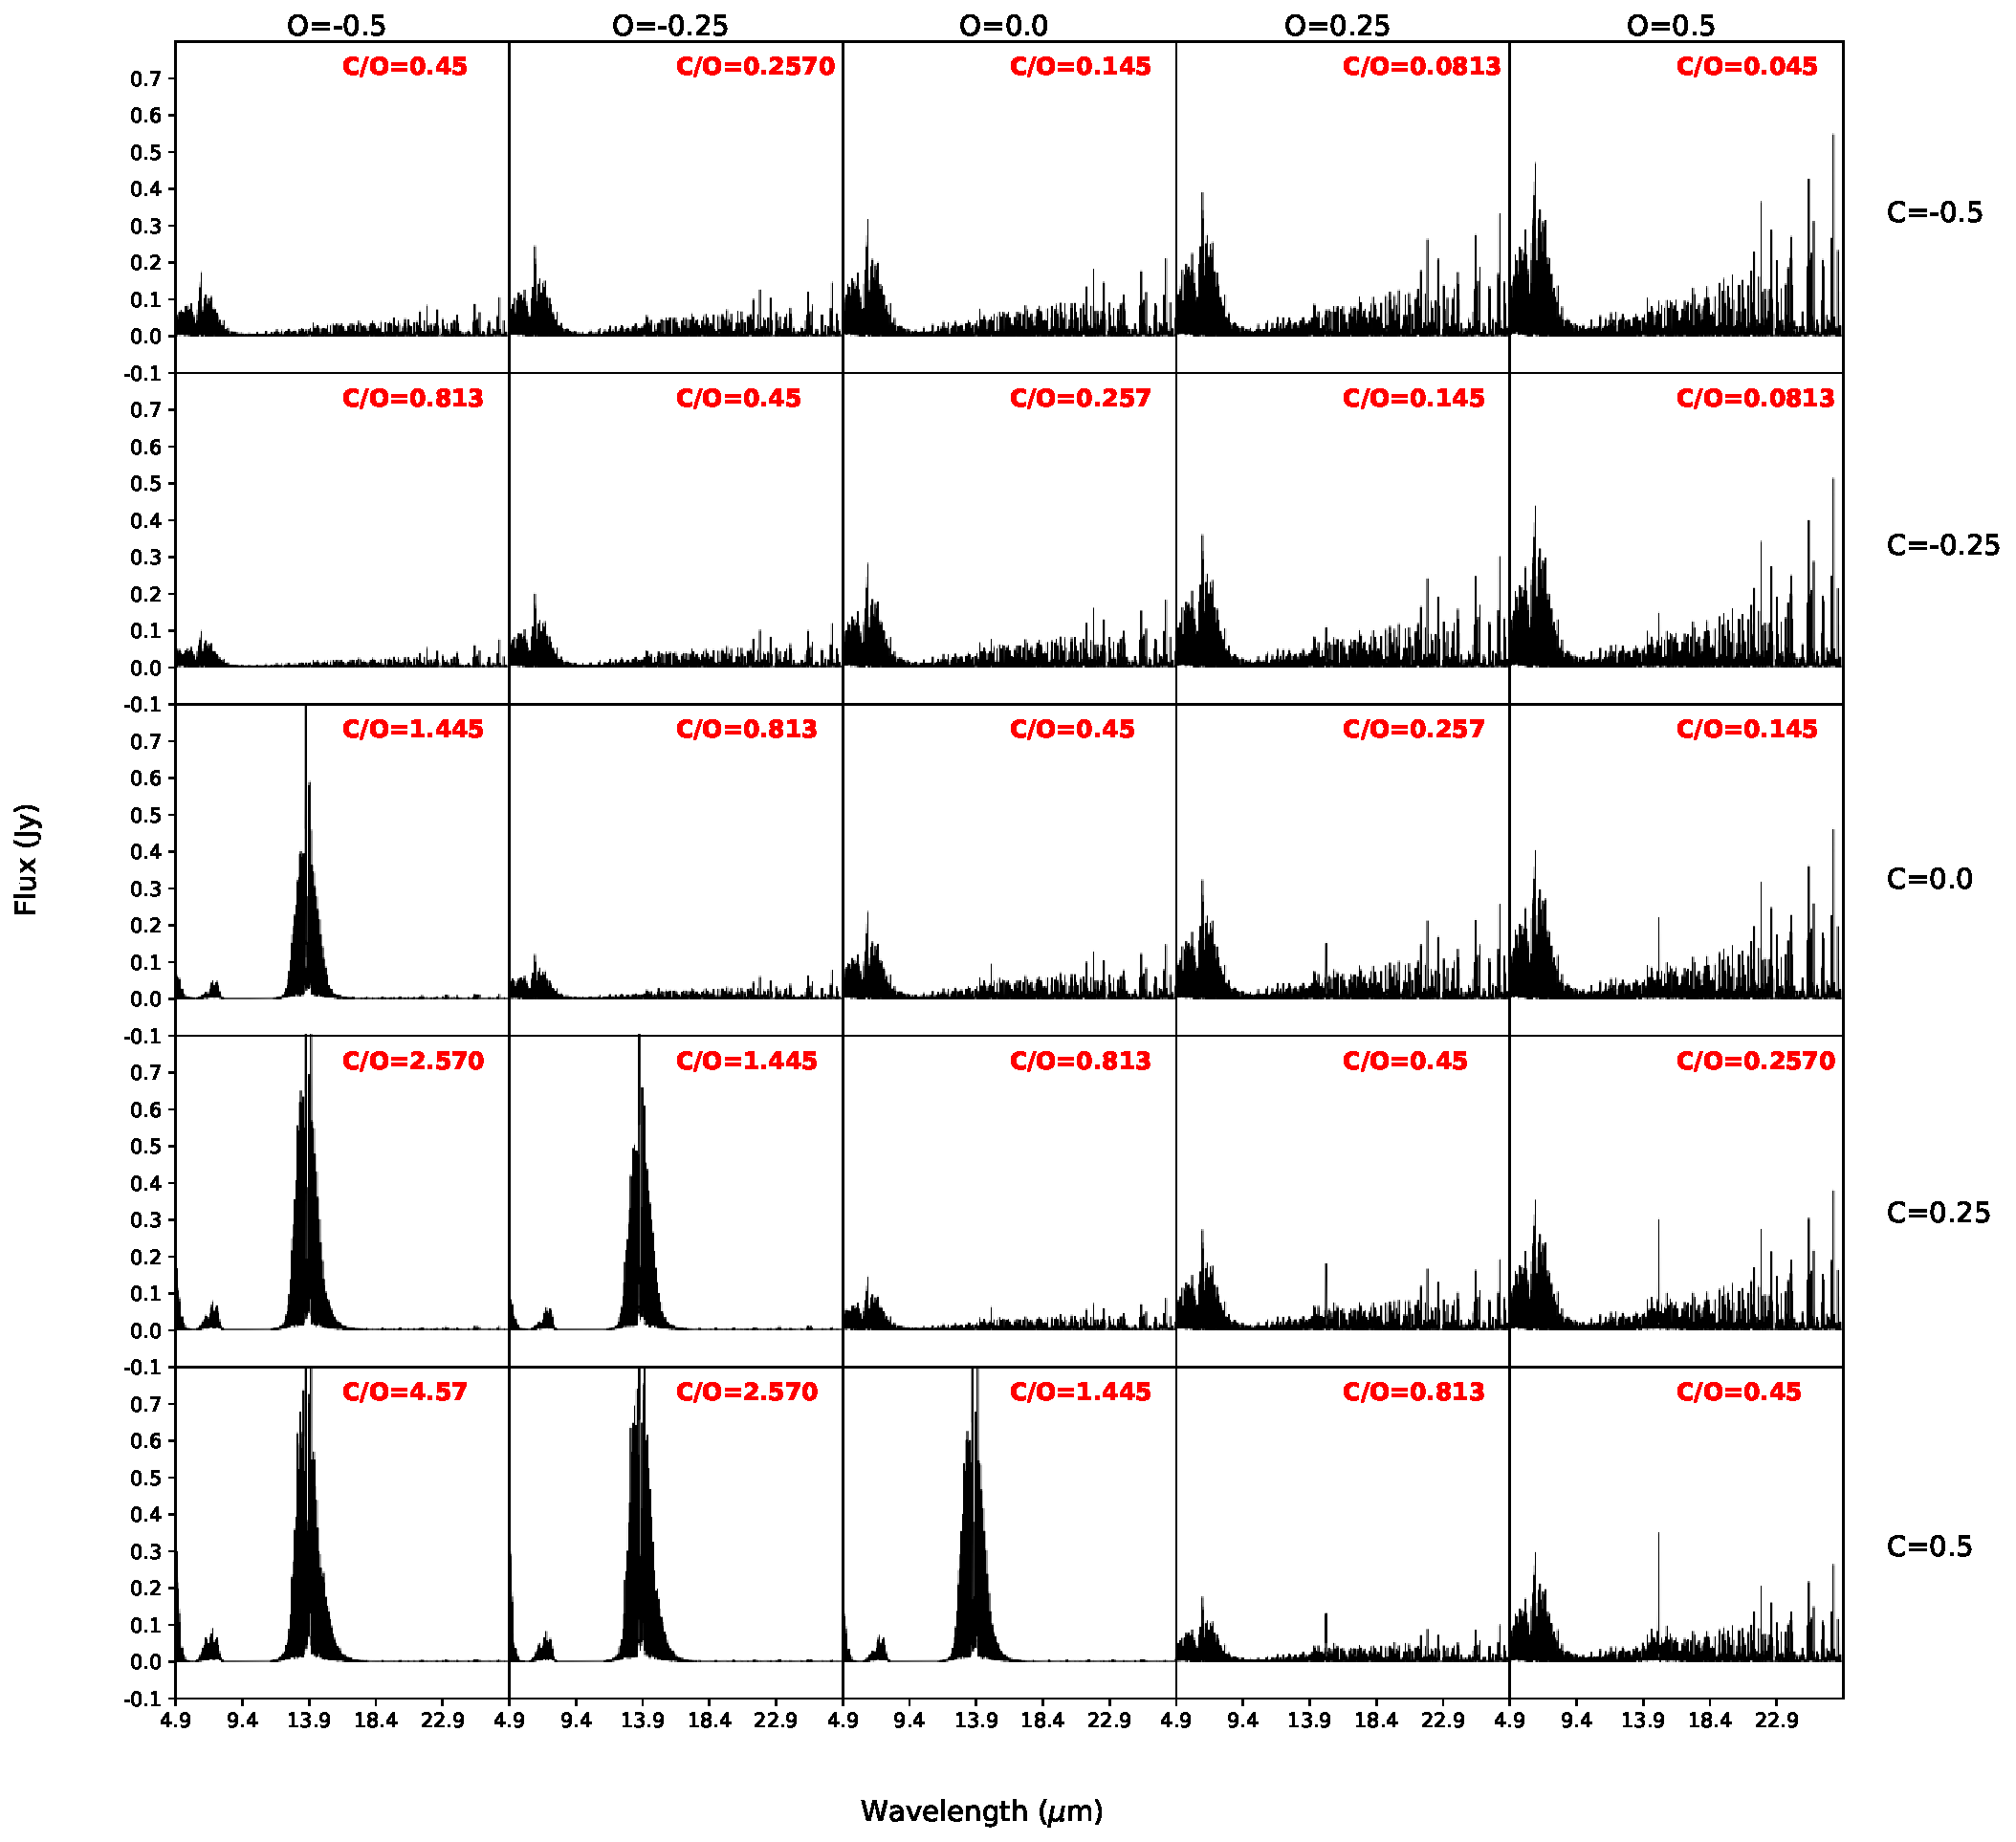
\includegraphics[width=\linewidth]{Figures/All_spectra.pdf}
    \caption{The simulated spectra of all the models in the model grid using FLiTs. On the horizontal axis, the O abundance is varied with -0.5 to 0.5 w.r.t. the reference abundance. The C abundance is varied with -0.5 to 0.5 w.r.t. the reference abundance from top to bottom.}
    \label{fig:all spectra}
\end{figure}
The flux of the different species changes depending on the abundances of C and O. In \ref{fig:flux HCN}, we can see this.
\begin{figure}[!ht]
    \centering
    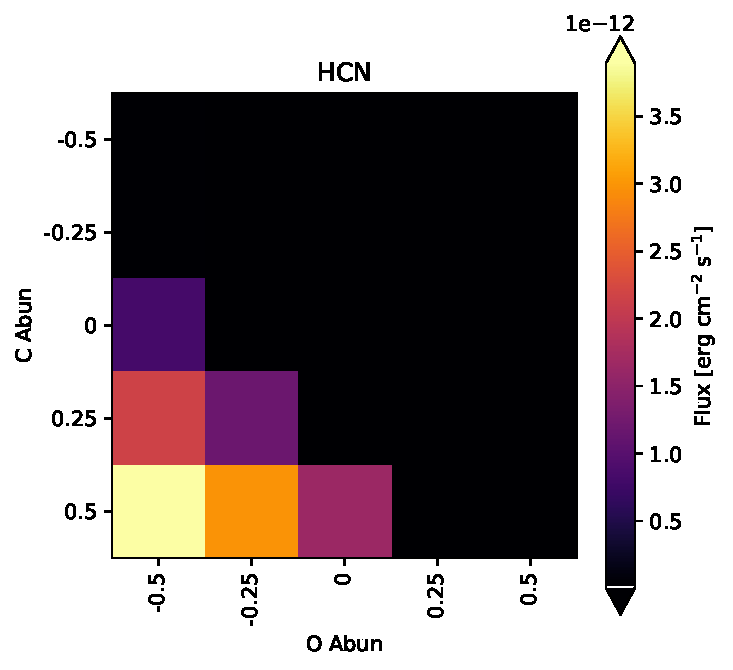
\includegraphics[width=0.5\linewidth]{Figures/HCN_heatmap.pdf}
    \caption{The total received flux of HCN for all the models in the grid.}
    \label{fig:flux HCN}
\end{figure}
\begin{figure}[!ht]
    \centering
    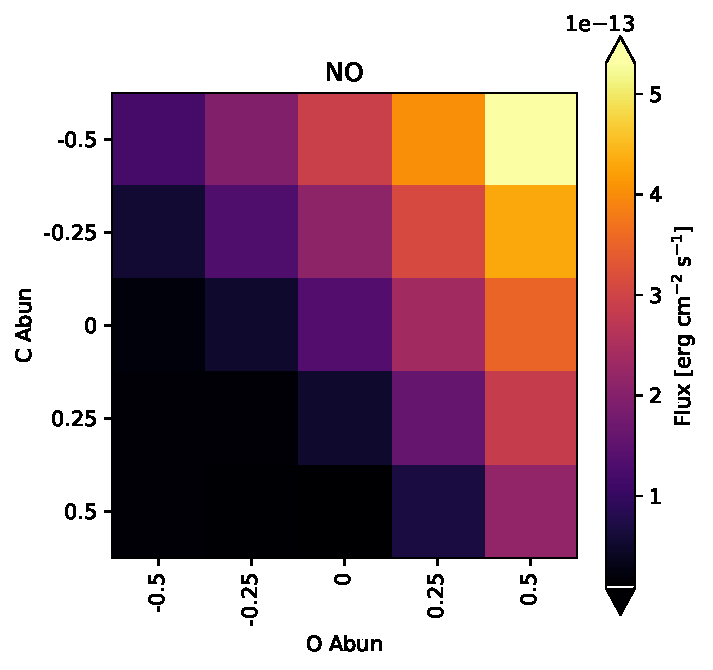
\includegraphics[width=0.5\linewidth]{Figures/NO_heatmap.pdf}
    \caption{The total received flux of NO for all the models in the grid.}
    \label{fig:flux NO}
\end{figure}
\begin{figure}[!ht]
    \centering
    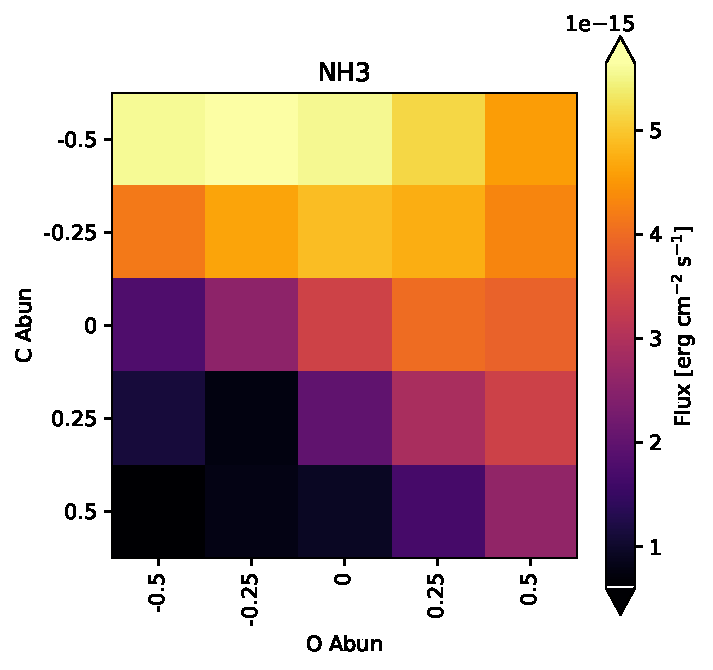
\includegraphics[width=0.5\linewidth]{Figures/NH3_heatmap.pdf}
    \caption{The total received flux of NH\3 for all the models in the grid.}
    \label{fig:flux NH3}
\end{figure}

The HCN increases as C/O gets larger, and NO decreases with it. The flux of NH\3 generally increases as the C abundance gets lower. We hypothesize that the reason for this is the reactions that take place to form NH\3.
We believe that OH is an important component in the formation of NH\3. 
\ce{NH2+ + OH -> NH3 + O+}
\textbf{MORE REACTIONS}

Next, we wanted to identify regions in the spectrum that could help us detect NO and NH\3. We split the model grid in 2 groups. One group has C/O smaller than unity and the other greater. We chose this distinction as the behaviors of the spectra is different. This difference is also visible in figure \ref{fig:all spectra). 
\begin{figure}[!ht]
    \centering
    \includegraphics[width=\linewidth]{Classification c/o>1.pdf}
    \caption{Caption}
    \label{fig:class>1}
\end{figure}
\begin{figure}[!ht]
    \centering
    \includegraphics[width=\linewidth]{Classification c/o<1.pdf}
    \caption{Caption}
    \label{fig:class<1}
\end{figure}
In both figure \ref{fig:class<1} and figure \ref{fig:class>1}
\begin{figure}[!ht]
    \centering
    \includegraphics[width=\linewidth]{NO region of interest.pdf}
    \caption{Caption}
    \label{fig:enter-label}
\end{figure}
\begin{figure}[!ht]
    \centering
    \includegraphics[width=\linewidth]{NH3 region of interest 1.pdf}
    \caption{Caption}
    \label{fig:enter-label}
\end{figure}
\begin{figure}[!ht]
    \centering
    \includegraphics[width=\linewidth]{NH3 region of interest 2.pdf}
    \caption{Caption}
    \label{fig:enter-label}
\end{figure}
All the spectra in figures \ref{} are without any noise. When we add noise to the spectra based on the methods described we get \ref{}. In this figure we see that the signal get completely washed out in the noise. So it would be hard to detect it. 
\begin{figure}[!ht]
    \centering
    \includegraphics[width=\linewidth]{Adding noise.pdf}
    \caption{Caption}
    \label{fig:enter-label}
\end{figure}

\section{Molecule Detection}

\begin{figure}[!ht]
    \centering
    \includegraphics[width=\linewidth]{cross-correlation.pdf}
    \caption{Caption}
    \label{fig:enter-label}
\end{figure}


\section{Application on Observations}

\chapter{Discussion}

\chapter{Conclusion}

\bibliographystyle{aa.bst}
\bibliography{references}
\end{document}